\documentclass{article}
%adds color
\usepackage{color}
%For diagrams
\usepackage{tikz}
%For inserting pictures
\usepackage{graphicx}
%For Code
\usepackage{listings}
%for dingbats
\usepackage{pifont}	
%margins
\usepackage{fullpage}
%todos add [hide] to ommit from output
\usepackage{todo}
\usepackage{lastpage}
\usepackage{url}

\synctex=1

\lstset{
language=C++,
basicstyle=\small \ttfamily,
commentstyle=\color{blue} \itshape,
numbers=left,
numberstyle=\footnotesize,
numbersep=4pt,
frame=single,
tabsize=2,
captionpos=b,
breaklines=true,
breakatwhitespace=false,
title=\lstname,
}

\usepackage{fancyhdr}

\def\ver{Version 1.1}

\renewcommand{\headrulewidth}{0pt} % remove lines as well
\renewcommand{\footrulewidth}{0pt}

\pagestyle{fancy}

\fancyhf{}
\fancyfoot[LE,RO]{\thepage\ of \pageref{LastPage}}
\fancyfoot[RE,LO]{--\ver--}


\fancypagestyle{plain}{ %
	\fancyhf{} % remove everything
	\renewcommand{\headrulewidth}{0pt} % remove lines as well
	\renewcommand{\footrulewidth}{0pt}
}

\synctex=1

%Allows me to use the matrix construct in tikz. Maybe I can delete this...
\usetikzlibrary{matrix}

%Gives me a simple way to make code looking words.
\newcommand{\comp}[1]{{\ttfamily #1}}

%About me
\author{Ben Seefeldt}
\title{An Introduction to Parallel Programming \\
		\small{\ver}}
\date{\today}

\begin{document}
\maketitle

\begin{abstract}
Parallel Programming is a powerful tool which can be used to drastically decrease the amount of time it takes to perform certain computations. This report will serve to outline some of the major themes in parallel programming. We will also take a look at three modern parallel languages to give an idea of how the concepts make the leap to actual implementations. \todo{Redo introduction entirely}
\end{abstract}

  \section{What is Parallel?}
  Parallel programming at its core aims to decrease run time by using multiple processors to do the same work that a single processor would normally do. Parallelism is a natural way to look at solving problems. Having multiple cashiers working at a Target makes much more sense than having a single worker who processes every customer one after the other.
  
  One of the main questions of parallelism then becomes how to divide work among the processors. This means ensuring that each processor is able to stay active and working on pertinent computations for the majority of the program execution.

\part{Concepts}

  \section{Flynn's Taxonomy}
  Flynn's Taxonomy is a way of classifying computer architectures which was created by Michael J. Flynn and is one of the traditional ways of explaining many of the differences between models. Flynn's distinctions lie in the number of instruction sets being run and on the amount of data being processed at a single point in time.
    \subsection{SISD}
    SISD or Single-Instruction-Single-Data is the hardware model that most computer scientists are familiar with. It is characterized by the von Neumann architecture. Instructions are loaded by the processor sequentially which operates on single pieces of data. One downside is that this model tends to make the assumption that data access time is an even cost, although this is far from the truth. Modern computers are constructed with many various levels of cache memory that take different amounts of time to access. Although some optimizations may take into account cache access, the basic model doesn't concern itself with the issue. This assumption can lead to much greater problems when transitioning to parallel programming.
    \subsection{SIMD}
    SIMD or Single-Instruction-Multiple-Data is a very common way to do parallel computing and is perhaps best utilized in scientific settings. CUDA, one of the languages we will be covering, uses a variation of this; specifically, Single-Instruction-Multiple-Thread\footnote{The difference being that a thread is not tied to a single piece of data}. these approaches work by sending the same instructions to a set of processors, each of which execute the instructions on different pieces of data. Although this may seem somewhat restrictive, it can be a very powerful tool. Many compute intensive programs cycle over a \comp{for}-loop where many of the computations can be run independently of one another. This makes SIMD and SIMT advantageous for large scientific computations that deal with things such as particle computations or graphics applications.
    \subsection{MIMD}
    MIMD or Multiple-Instruction-Multiple-Data is the way that most people tend to think about parallel computing. In this model, multiple processors perform different tasks on different pieces of data. A good example would be a farm with many workers. Each performs different jobs throughout the day. One may be maintaining equipment while another lays drainage tile. This can be a very powerful model when implementing a solution using data-pipelining, where single pieces of data move through a series of processors each working on a particular aspect of the problem, much like a car assembly line.

  % \section{Parallel vs. Serial}
  % Many problems that seem relatively simple using standard serial programming techniques become much more complex when approaching them in parallel. Many of these problems can fall under one of two main issues: communication or memory access.
	% \subsection{Communication}
	% When managing large amounts of workers, keeping them organized and productive is the supervisor's main concern. In parallel programming, the programmer plays the role of supervisor for a group of threads. The best way to maintain this organization is having some method for the threads to communicate to each other their position in the code. Certain solutions to this problem
	% \subsection{Memory Access}

  \section{Algorithms and Common Constructs}
  There are many different parallel hardware configurations and even more parallel languages. Fortunately for programmers, there are many common constructs between all of these. The general problems and accepted solutions are relatively universal. This allows us to study a relatively small number of concepts and gain a basic understanding of most of the languages. After this, we will look at the specifics of three languages to see these concepts in action.
	\subsection{Threads}
	Many languages use \emph{threads} to organize processors. A thread is the most basic unit of parallelism, and can be thought of a single processor running some piece of code. Typically parallel program will \emph{launch} or \emph{run} a certain number of threads either with every piece running the same code (SIMD) or separate threads working on different problems (MIMD). Threads are typically allowed to communicate with each other through a handful of different methods depending on the specific language. Much of our discussion about parallelism will focus on threads and their organization.
	
	\subsection{Latency and Throughput}
    When trying to increase performance two major issues are latency and throughput. Latency is the amount if time it takes to complete any particular block of work. Throughput is the amount of work that can be completed in every unit time. \todo{Add picture illustrating this fact.} Much of the work of parallelism is an attempt to increase throughput. Doing more work in less time is the ultimate goal of parallel programming. Understanding how speed can come from two separate aspects of a program can help in designing quicker and more efficient programs.
	
	\subsection{Amdahl's Law}
    Amdahl's law is an equation explaining how much a performance gain we can expect from parallelizing any particular problem. It makes common sense that parallel speed up will be limited by the amount of sequential code that is necessary for the computation. If we assign $S$ to the speedup gained, $N$ to the number of processors, and $\beta$ to the percent of total time time it takes to do the serial aspects of the program, Amdahl's Law can be formulated\footnote{From {\it Introduction to Parallel Computing} by Ted G. Lewis and Hesham El-Rewini.} as:
    $$S=\frac{N}{\beta N+(1-\beta)}$$

    Amdahl's law typically gives some very pessimistic results for parallel improvement. \todo{Add in a results table: May be merged in with G-B Law results below.} Following this algorithm, it seems as though most problems would be severely hindered by even medium or small sequential portions. However in 1988 a Sandia research team completed a parallel implementation that achieved much better results than Amdahl's law predicted. They were able to rewrite Amdahl's law into Gustafson-Ban's law, which more accurately describes parallel speed up.

    \subsection{Gustafson-Ban's Law}
    The heart of the difference between these two equations is the relationship between $N$ and $(1 - \beta)$. This relationship can be best understood as the fact that as the number of processors increases or decreases, the amount of time it takes to do the problem will change. By neglecting this fact, Amdahl ended up with much more pessimistic results. John Gustafson and Ed Barsis found that these two terms are virtually never independent of each other. By changing this assumption, they reformulated\footnote{From {\it Introduction to Parallel Computing} by Ted G. Lewis and Hesham El-Rewini.} the equation as:

    $$S = N - (N - 1)\beta$$

    This rule will consistently compute more speedup than Amdahl's law, which more accurately represents the gains that parallel can offer.
    
    \subsection{Atomics}
    Before understanding what atomics are, it is important to understand the problem they attempt to solve. Let's look at an example where a problem might arise. Imagine two threads, A and B both working on a single integer, \comp{x}. They both must execute a command \comp{x++}. The way a single increment occurs on a processor is three parts: the value is loaded from memory, incremented on the processor, and then stored back. When dealing with a serial processor these actions are performed one after the other every time an increment must occur. However when dealing with multiple processors a particular order is not guaranteed. Let's think about the situation we were looking at with threads A and B. They both need to run all three of the parts. Let us imagine that \comp{x} is initially equal to 4. A loads \comp{x} which it saves as 4. B immediately loads the values as well, which is is also 4. Thread A increments the value to 5 and stores it back into the variable \comp{x}. Thread B increments its original value of 4 to 5 and stores the 5 to variable \comp{x}. The final value of \comp{x} ends at 5. This is incorrect, 4 incremented twice should be 6.\todo{Add an illustration showing this.}
    
    This is the issue that atomics serve to solve. An atomic operation is one that must act as though it is completed in one step. Most languages have built in atomic operations. Athough built in atomic operations may seem like a quick fix, they can lead to many problems that may end up making a parallele solution slower than its serial conterpart. In the next section we will cover resource contention, a problem that can severely slow down a solution that uses atomics in the wrong places.
    	
    \subsection{Resource Contention}
    \label{sec.rescont}    
    We've mentioned resource contention  before and how it can severely slow down programs. Even thought atomics and locks (which we will cover in a future section.) allow us to write programs where individual threads don't mess up the data computed by other threads, it can still slow down computation. Why is this? It boils down to resource contention. If you are attempting do a trivial example such as counting the number of 5's in an array. A simple way to do this would be a for-loop with a conditional that tested if the current element was a 5. If the contitional returns \comp{true}, we increment \comp{num} once.

    A simple way to do this in parallel would be to launch as many threads as there are elements in the array and have them each do a test: if it's element is five, increment a global \comp{num} counter. Due to the problems we had with multiple threads attempting to increment the same variable. This may lead us to use atomics to solve the problem. However, all the threads are attempting to use the atomic operation at the same time. In the end, the threads are forced to update the variable in a serial manner, one right after the other. There would be no speed-up, in fact the execution would be slower than the standard serial program due to the overhead associated with initializing the threads.
	
    If a program isn't designed intelligently, resource contention can slow down a program so much that it can overshadow any of the gains from parallelism. In section \ref{sec.pairwise}, we will look at one potential way to solve the problem we just looked at to increase speed.
	
	 \subsection{Synchronization}
    In many cases threads can work along side each other without the need to interact. Computations that do not require interaction between any of the threads are referred to as ``embarrassingly parallel computations''.

    However, many times, this is not possible. It is necessary for threads to send data to each other, or at least tell each other where they are in the program. This is where synchronization comes into play. Most parallel programming languages include a method that creates a barrier which stops all threads until every thread reaches that point.\todo{Expand section}

	
    
    \subsection{Locks}
    Locks solve a very similar issue as atomics. Locks are objects or variables that can stop a thread from moving to a certain point in the code. Although there are many different variation, the basic idea of lock is simple. A thread can `acquire' a lock which prevents other threads from acquiring the same lock and progressing beyond it in the code.

    The difference between different locks typically lie with how the lock takes care of requests for the lock after it is already owned by a thread. Different options include queuing based on which requested first, based on job size or other variables.

    The biggest worries when dealing with locks is running into deadlock. To illustrate this, we'll look at two threads that need to deal with acquiring locks, lets say threads C and D and locks J and K. At this point in the program execution, imagine that thread C has acquired lock J and D has lock K. However, in order to move forward with program execution, thread C must acquire K and D must acquire J. The program is stuck in deadlock and will never continue. Because parallel execution varies on different runs, it is sometimes hard to locate deadlock issues. Similarly with atomics, resource contention can become an issue.
	
	\subsection{Pair-Wise Summation}
    \label{sec.pairwise}
    Next we will look at one of the simplest ways a large amount of numbers can all be added together without worrying about resource contention and other such nasty things. Pair-wise operations are a rather simple concept. The operation is applied by numerous threads, which half in number after each iteration. The major limitation to any pair-wise operation is that the operator must be associative. Let's look at a simple example with an 8 element array in figure \ref{fig.spws}.

\done\todo{position}
    \begin{figure}[!h]
    	\label{fig.spws}
    \begin{center}
    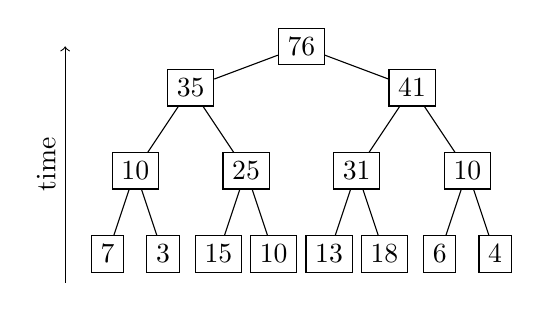
\begin{tikzpicture}
       %\draw (0,0) ]- (0,15);
    [every node/.style={rectangle,draw},level 1/.style={sibling distance=80pt, level distance = 15pt},level 2/.style={sibling distance=40pt, level distance = 30pt},
    level 3/.style={sibling distance=20pt, level distance = 30pt}]
      \node at (-2,5) {76}
        child{ node {35}
          child {node {10}
            child {node {7}
            }
            child {node {3}
            }
          }
          child {node {25}
            child {node {15}
            }
            child {node {10}
            }
          }
        }
        child{ node {41}
          child{ node {31}
            child{ node {13}
            }
            child{ node {18}
            }
          }
          child{ node {10}
            child{ node {6}
            }
            child{ node {4}
            }
          }
        };\draw [->](-5,2) -- (-5,5)
        node[above,rotate=90,style={rectangle,draw=none},midway]
        {
          time
        };
      \end{tikzpicture}
      \caption{A simple pair-wise summation.}
      \end{center}
    \end{figure}

    This kind of a solution can be implemented in many different ways depending on the specific programming language. Some depend on global memory, while others use message passing interfaces to send data from one thread to another. Some languages have a function to do this sort of operation automatically. This will be covered in section \ref{sec.reduce}.


    \subsection{Prefix Sum}
    \done\todo{Redo the introduction to this section.}
    The prefix sum is a rather unnecessary construct in serial programming, but is vitally important in parallel programming. This operation is also known as a scan in many implementations. Imagine we have a series of numbers, $x_{0}, x_{1},...x_{n}$. The result of a prefix sum into an array $y$, is equivalent to, $$y_{i} = \sum_{j\leq i}^{} x_{j}$$, or the sum of all the numbers up to the current index. There are two variations of the prefix sum, exclusive and inclusive. An exclusive scan begins with a 0 and \emph{does not} include the current index. (This means the final entry, $y_{n}$, is one less then the sum of all numbers in the array.) An inclusive scan \emph{does} include the first number, and ends with the sum of the array in the final position.

    But how do we compute this? In a serial implementation, an efficient solution is trivial. Very rarely is such a computation even necessary. However, in parallel we are faced with a very difficult problem. Every element depends on the elements before it. It seems to demand a serial solution. But fear not, a clever algorithm allows for a parallel solution. One way to do this is by combining the pair-wise summation that we did in section \ref{sec.pairwise} with a downward sweep phase. Imagine that after the initial sweep up we move back down the tree following three simple years. We send the identity (1 for multiplication, 0 for addition) to the first root. We send the value from the parent to the left and send the sum of the parent and the left child to the right child. In this image, we already have completed the pair-wise summation. The computation has taken place inside an array of integers, which means all of the partial sums are still in the array. Figure \ref{fig.psc} shows this in action.

	\begin{figure}
		\label{fig.psc}
    \centering
    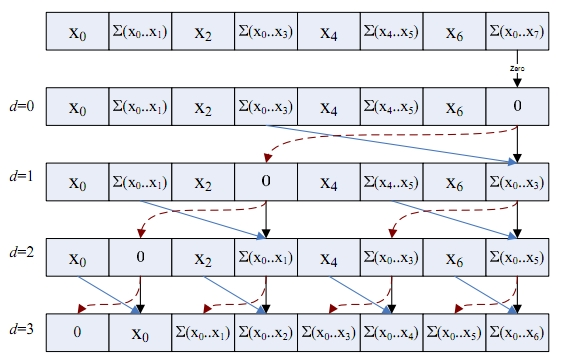
\includegraphics[scale=.65]{pic/PrefixSum.jpg}
    \caption{A prefix sum computation.}
    \end{figure}


    Although it may seem like an inefficient way to do the computation (doing the pair-wise first), but the gains from parallelism in a well written algorithm can overshadow the excess computation and in the end make the computation more efficient. How can we use this algorithm to help us create better parallel programs? The results from a prefix scan can be used to help organize data using scatter-gather which is covered in section \ref{sec.sg}.





    \subsection{Batcher's Bitonic Sort}
      I spent a considerable amount of time examining Batcher's bitonic sort, which we will look over because it provides a good example of how to write an efficient parallel algorithm that can solve a problem that would normally seem inherently sequential. Batcher's sort is perhaps best understood with an example before explaining. 
      
     \done\todo{check size}
    \begin{figure}
    \centering
    \includegraphics[scale=.85]{pic/bitsort}
    \caption{A simple pair-wise summation.}
    \end{figure}

    The sort cycles through two variables $p$ and $d$. Variable $d$ increments up to 3 with $p$ beginning at $d-1$ and moving downward to 0. Both variable dictate a certain movement in the sort. $p$ is which bit location pairs are created with. For example, when we have $(1,2)$, the 1 tells us that threads that differ \emph{only} by the position 1 are paired. $d$ tells us which bit to look at for direction. If the $d$ bit for a given pair is 1 we sort ascending and if it is 0 we sort descending. It is worth the effort to work through the sort. It is a very interesting algorithm and it is exciting to work through it and see how it all works out.



    \subsection{Scatter-Gather}
    \label{sec.sg}
    One large problem we are forced to deal with in parallel programming is threads that have different amounts of work to do. Sometimes threads doing different amounts of work can severely slow down execution time.\footnote{This becomes a large issue with the way CUDA handles objects called threads warps.} To help visualize why this would end up being an issue, imagine a sparse vector on which we would like to do some computation on each piece of data. If only $\frac{1}{200}$ of our element positions are filled, we can lose a large amount of time trying to test if there is an element present before moving forward on the computation. Scatter-gather is a wide label to describe a class of algorithms that serves to reorganize or re-index data so it can be accessed more efficiently. Different implementations take different things into account, but the main idea is to end up with data in a more compressed way.

    \subsection{Reduce}
    \label{sec.reduce}
    We have already covered the majority of algorithms necessary to create a good reduce function. A \emph{reduce} in parallel programming is the process of applying a single associative operator to all piece of data in a set. A simple example would be the sum of an entire array. Both addition and multiplication are common for a reduce function. But others like \comp{min} and \comp{max} are also commonly used. The solution we used for the pair-wise summation in section \ref{sec.pairwise} is a commonly used solution for doing any reduce operation. Several of the languages that we are going to cover will have built in reduce functions which leave the programmer to fill in the specifics of the operation. 

   % \subsection{Pipelines}
    %\label{sec.pipe}
    %More research needed.
    %Along with scatter-gather, there are other tools that can be used to decrease the amount of idle time and increase speed. Pipelining is one of the tools many languages use. Pipelines are used to keep jobs in a que

    \subsection{Cache Conflicts}
    It is important to keep in mind the way hardware accesses data, as it can have a sizable impact on the speed of a program. One way that hardware designers have increased speed is by adding a cache on chips which allows for temporary storage of data that can be accessed quicker than a hard drive. However, one issue that can come up is cache lines conflicts where two pieces of data are put on a single cache line and if they are accessed back and forth numerous times, cache misses can severely slow down execution time. Although many languages will take care of these issues from the beginning, it is very helpful to be aware of the concept.

  \section{Parallel Models}
  There are many different ways to implement parallelism, depending on the exact specifications of the hardware. One interesting aspect of parallel computing is that there is no dominant model. We will begin by looking at RAM, the dominant model for sequential programming before looking at several parallel models.
    \subsection{RAM}
    We will spend little time on the RAM model (characterized by the von Neumann architecture) and assume that most people reading this are familiar with the general model for execution.
	
	The RAM model is characterized by the famous von Neumann architecture. Most computer scientists should be intimately familiar with this model as all sequential programming is done using it. The general format is stepping through a program bit by bit, putting a single instruction in the processor, executing and then incrementing the counter in order to move to the next instruction.
	
	The general RAM model also makes the assumption that all memory access is an equal cost, which is far from the truth. We have already mentioned that hardware designers have created elaborate systems of cache memory that allow for speedier memory access. Realizing the mechanics behind these systems and writing code that takes it into account can drastically decrease execution time.
	
    \subsection{PRAM}
      PRAM is a basic variation (the `P' stands for parallel) on the RAM model that tries to add parallelism `on-top'. However, it inherits the major weakness of the RAM model. The most serious problem in dealing with parallel in this way is the inconsistency in the memory access patterns. All memory is accessed in the same way by all of the threads. Problems such as resource contention can cause very big problems. Although simple locks can solve some of the problems there are many more complex and better ways to solve them. Another issue that has to do with cache memory. In the RAM model, memory access, particularly cache access, is never explicitly dealt with. However, in parallel, very small increases in speed can be vital to creating an efficient program.
    \subsection{CTA}
    CTA is the Candidate Type Architecture. It is an attempt at a standard way of organizing processors. The basic outline is $n$ number of processors connected via an interconnection network. There is also one processor denoted as the `controller', which helps dictates the actions of all of the other processors.
	
	\done\todo{check size}
	\begin{figure}[h]
    \centering
    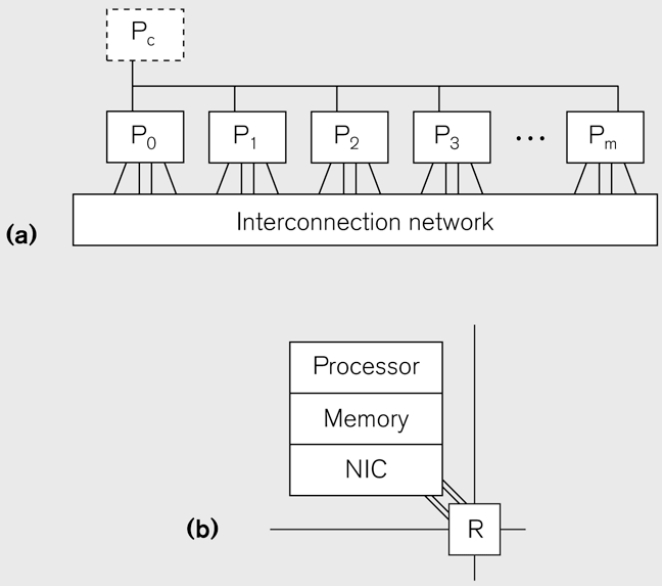
\includegraphics[scale=.45]{pic/CTA.jpg}
    \caption{A visual representation of CTA.}
    \end{figure}
	
	The standard does not outline a specific network, but rather allows it to change depending on the implementation. Different network topologies can help to decrease computation latency. The last thing to take care of is {\it communication} between the specific threads. There are three main ways to doing this.

      \subsubsection{Shared Memory}
      Shared memory is an easy to understand model. It naturally extends the PRAM model. All processors access the same space of memory. Like the PRAM model, we can run into issues with resource contention. However we do have tools to deal with this, and many times the advantage given by the CTA processor organization can help overcome those issues. One nice part of this memory model is that it presents a single memory picture to all of the threads.\done\Todo{Redo this whole section.}

      \subsubsection{One-sided Communication}
      One-sided communication is a memory model that is based off the shared memory model, but relaxes some of the hardware specifications. Where shared memory demands the single memory image, one-sided communication does not. It shifts the burden from the hardware to the software and forces the programmer to work harder to ensure the correct data is being used. \done\todo{Elaborate}

      \subsubsection{Message Passing}
      Message passing is a completely different beast than the first two and does not rely on shared memory space at all. \done\todo{Rephrase}Instead, threads are only allowed to access their privately held memory. Sharing between threads is done via messages. Both the sending thread and the receiving threads must have coded into their execution order the fact that a message will be passed. This is a very common model and has many advantages.

\part{CUDA}
CUDA is a language release by graphics card manufacturer Nvidia that allows programmers to write code that can be directly executed on GPUs. The language consists in simple extensions to the C++ programming language. This makes it relatively easy for a programmer who has a knowledge of C++ to write parallel code. Thinking back to Flynn's taxonomy, we can classify CUDA in a way that is not actually in Flynn's original taxonomy. CUDA is considered SIMT or single instruction-multiple thread. This is similar to SIMD, except that instead of having each process tied to a single piece of data, each thread is given a thread ID that can be used to do a much wider range of computations. The general format of a CUDA solution is copying a data set to the GPU, launching a kernel on the data, having each thread deal with a single element or range of elements and repeating kernel launches until a solution is reached. If some of these terms don't make sense, don't worry, all will be explained in good time.

	\section{Threads, Blocks and Grids}

    CUDA is organized in a hierarchical model that is all configured by the programmer at launch time. This can be used to make even more efficient programs if the programmer takes the time to do testing to find the most advantageous configuration.\footnote{The other languages we are going to look at don't demand the programmer takes care of this configuration, instead it is left up to the compiler which attempts to come up with the best one on the fly.}

    The thread is the basic unit of computation in CUDA. Conceptually it can be thought of a single serial processor working through one sequence of commands. On the hardware side a thread is a single ALU that is part of a row of ALU's that share a single controller. Threads are then grouped into \emph{warps} which is a group of 32 threads. Warps are important because all threads inside a warps follow the same execution order. A kernel that had conditional statement, \comp{if(threadID\%2==0)} would force each thread to work through the steps for both possibilities of the conditional, even if not every one is supposed to. Keep in mind that this would not change the eventual answer as each thread will only end up \emph{actually} executing the correct path. However programming with warps in mind can help to give a program just that little extra boost.

    The next level up in the hierarchy is the \emph{block} which is a grouping of threads, typically in some logical relationship with the problem set. The maximum number of threads in a block depends upon the revision number of the graphics card. The GeForce GTX 285 cards in beefy both allow for a maximum of 512 threads per block. Newer models have support for 1024 threads per block. Blocks can be visualized as a three dimensional group of threads with the maximum dimensions of 512x512x64 in any configuration that does not exceed the maximum number of threads. Blocks are unique to the CUDA architecture and form the core of the setup of solutions. Blocks must be thought of as completely independent from each other. The execution order between blocks is not strictly defined. Threads of the same block also have a single shared memory area which provides much faster read and write times then the global memory. Also, thread communication is limited to threads within a block, which is something we cover in section \ref{sec.synchronization}.

    Blocks are organized into one higher organizational unit. A \emph{grid} is a two dimensional collection of blocks. The maximum dimensions are again dependent on the revision number of the graphics card. The beefy cards allow for a max grid size of 65535 by 65535. A single grid runs at one time and completes before another kernel launch takes place.
	
	\section{Kernels}
    The kernel is the piece of code that actually runs upon the GPU. It is a method that is marked in the code with a \comp{\_\_kernel\_\_}. It is then \emph{launched} by the programmer with specific parameters that tell the number of blocks and threads.

    Typically a kernel will define an order of execution that works on pieces of data based on the thread ID. The most common way to get a thread ID is using the formula, \comp{blockIdx.x*blockDim.x+threadIdx.x}. This gives every thread a unique ID number which can be very helpful if you have an array of numbers all of which need to have a certain operation performed upon them. The \comp{x} can be replaced with \comp{y} or \comp{z} depending on if you used two or three dimensional launch parameters.

    \section{Memory Spaces}
    As we covered in general concepts one of the most important considerations in parallel programming is how to manage the memory spaces we have effectively. In the three languages we are going to look at it is perhaps most important in CUDA, which has many clearly defined memory locations, all with their own strengths and weaknesses.
      \subsection{Register and Local}
	  The register and local memory locations are both accessible from only a single thread and information can not be shared unless copied into another memory location. In a program, these would typically be used for temporary variables that aren't part of the final solution. \todo{Look up difference between the two.}
      \subsection{Shared}
      Shared memory is much quicker then global memory, and whenever computations are going to be done on a group of numbers, it makes sense to copy data into shared memory before continuing. Shared memory is accessible only between threads of the same block. This makes it slightly more difficult to program with. Unlike traditional serial solutions, you don't have access to the entire data set and must work a solution that does not require it.
      \subsection{Global}
      Global memory is accessible by any thread in any block. It is also the main memory location that is accessible by non-GPU code. Data sets are copied from the computer to the global memory. When a kernel has been launched it is typically a bad idea to manipulate data which is still stored in global memory. It is the slowest of all memory locations. All data that is used by the GPU \emph{must} be placed into global memory. This requires a serial copy executed by the CPU. CUDA offers two commands used for moving data to and from the GPU. In the following example variables preceded by \comp{d} are device (GPU) pointers and those with a \comp{h} are host pointers.
	  \begin{lstlisting}
//To copy from CPU to Global Memory.	
cudaMemcpy(d_graph_nodes_input, h_graph_nodes_input, num_elements*sizeof(float),cudaMemcpyHostToDevice);

//To copy back from Global Memory to CPU.	
cudaMemcpy(h_graph_nodes_result, d_graph_nodes_result, num_elements*sizeof(float),cudaMemcpyDeviceToHost);

//Both commands take inputs: destination, origin, size of copy, direction.
	  \end{lstlisting}
	
      \subsection{Constant and Texture}
	  Constant and texture memory locations are specific to the GPU hardware we are working on. The motivation for this memory space is high performance game graphics. Both allow values to be loaded in prior to execution that can be quickly accessed by all threads. However, threads are not allowed to modify these areas. In games this would allow a texture model to be quickly accessed and there is no need for it to be accessed. I did not have much experience using this memory in my solutions.




    \section{Synchronization}
    \label{sec.synchronization}
    Thread communication and synchronization are limited in CUDA to threads in the same block. The main CUDA command used to synchronize threads is \comp{\_\_syncthreads()}. In a piece of code this command will stop all threads in the block at that line until all of the threads reach the line at which point they all continue.

	\section{Atomics}
    CUDA also has built in atomic functions for devices version 1.1 and above. They act like atomics normally do. The exact specifics of which functions are supported can be found in the CUDA documentation. Keep in mind that there are many downsides to using atomics that can slow down execution. Before using an atomic it is typically better to look for a solution that needs less of them.



  \section{Thrust}
  Thrust is a library of code that contains standard solvers for many parallel problems such as reduce and scan. It also contains new data structures that can provide faster memory access due to their correct alignment. Thrust can be very helpful because it allows the programmer to focus on the design of the program instead of being mucked down the by the particulars of CUDA and being forced to re-implement common solutions for every problem. I used Thrust sparingly in my programs, choosing instead to focus on working through the common solutions in order to gain a better understanding of standard parallel constructs.


  \section{Example Code}
  \subsection{PageRank}
  Let's take a look at an entire CUDA program and see what we've been talking about in action. Make sure to look at the comments, they will give you an idea of what's happening along the way. We will start at the top, and like a `Choose Your Own Adventure Book' we'll skip around through the code by following line numbers.
  
  \lstinputlisting{code/mp1-part3.cu}

  This is obviously a very long and complicated program for someone who has never worked with the language before. However a solid understanding of C++ makes the code much more understandable. The comments should help to make light of most of it. Fortunately there is also a serial implementation to compare to the parallel code. On execution, the program also outputs the speed of each execution. The parallel implementation takes around 973ms, while the serial code takes 14862ms. Thats around 15 times faster!

\subsection{Black-Scholes}
  We're going to look at one more example, this time with multiple files. We will use some Thrust code so we can see it in action. The following program will compute multiple interations of the Black-Scholes algorithm. Black-Scholes is a financial algorithm that is used to compute \emph{calls} and \emph{puts}. A call is an agreement that gives an investor the right to buy a specific security at a certain time at a certain price. The financial options will be stored in a series of arrays that hold stock price, option strike and option years. A single option can be found by using the same index position in all of these arrays. We will also be using a parallel pattern called \emph{compact} in order to speed up computation. Black-Scholes is run multiple times on the same data set. However, after the first execution a large number of data points are eliminated from future computations. Instead of running over sparsely populated vector, we use compact to `squeeze together' the remaining data points so future computations will be quicker. We will accomplish this using both scan and scatter algorithms, all of which are contained in their own files. There will be line references that should help you to follow through most of the code.

  We will start with \comp{black\_scholes.cu} which contains the functions for computing the Black-Scholes results. Follow the code through from top to bottom.

  \lstinputlisting{code/black_scholes.cu}

  Keep in mind these are just helper functions that we will use in the final implementation. Now let's take a look at the scan implementation. For this, I chose to use Thrust in order to have a highly efficient implementation.\footnote{I attempted to do my own implementation, and although I was successful in creating a working version, the speed-up was not as high as Thrust, which led me to choose their code.}

  \lstinputlisting{code/scan.cu}

  Next we're going to cover the scatter code. We mentioned scatter in section \ref{sec.sg}. This code will be used in the compact algorithm, which is the way we are going to get a large amount of speed up from our code.

  \lstinputlisting{code/scatter.cu}

  Last, but certainly not least is the code for the compact. This will use both the scan and scatter methods to compact the options so that our subsequent runs will be quicker.

  \lstinputlisting{code/compact.cu}

  The last thing we need to do is put all of this together into a runnable program with a \comp{main} method that we can use for actual problem solving. Although it looks as though there is a lot of complex code, most of it is data allocation, copying and terminal output.

  \lstinputlisting{code/mp3-part3.cu}

  Let's take a look at what this code output, so we can see what kind of speed we are getting.

  \lstinputlisting{code/output.d}

	We can also run the same code and see the speed \emph{without} compaction.

  \lstinputlisting{code/output2.d}

  We get close to \emph{doubling} speed up by using compaction. Note, however that compaction takes 24.3ms. This is overshadowed by the 16ms we save for each of the five subsequent rounds. If we were running less options, or if compaction took more time, we could in fact slow down the computation overall if we are not careful. Another important slow down to notice is the time for the data copy. Copy time for this program is 35.5ms. The time required for this copying means that the longer the data can stay on the GPU the better. Serial code does not have this disadvantage and so for smaller computations on large data sets, serial code will sometimes complete faster.

  This should give the reader a good idea of how CUDA works and some of the strategies behind computing on an Nvidia card. We haven't covered some things such as logical grouping of 3 dimensional data sets or binning, two things that can help when doing particle computations.\footnote{More examples may be added as time permits.}

\part{Intel TBB}
Intel's Thread Building Blocks is a much different look at parallelism from that of CUDA. CUDA demands the user explicitly create all parallelism through the use of kernels that are launched with user defined thread sizes. TBB takes a much more laid back approach in an attempt to make parallelism easier to add to a project without as much elbow grease as CUDA. TBB accomplishes this by having parallel templates built into the language. In CUDA simple problems must be reimplemented every time they are used.\footnote{This can somewhat account for the popularity of Thrust.} TBB has template function in which the programmer provides the specifics for their implementation. These templates are implemented by filling out methods in a class, which is passsed to a method provided by TBB. 

  \section{Working in Parallel}

  For example, in order to perform a parallel reduce the we need to split data, perform certain calculations and then join the data back together. The TBB specifications ask us to define a a class that contains methods for these operations. Our class \comp{SumFoo} should take care of this for a simple reduction algorithm. Let's look at some code to see this in action. 

  \lstinputlisting{code/reduction.d}

  However, this is just a simple class definition, how would we use this code in a practical circumstance? Below are two methods that would perform the same operation, first in serial, and secondly in parallel using the \comp{SumFoo} class.

  \lstinputlisting{code/run-reduction.d}

  As you can see the overall code is much simpler then CUDA syntax. After an class is created that contains the correct methods. In this case \comp{operator}, \comp{join} and constructors. Then, after creating the object with the data, the standard \comp{parallel\_reduce} method is run, passing in the object and the size of the data. The \comp{parallel\_reduce} method calls the \comp{operator} method in the \comp{SumFoo} class. After this, TBB takes care of the rest. It will automatically calculate the launch parameters. This makes parallelism much easier to apply. As you can imagine, reduce is not the only operation that TBB supports. Other operations such \comp{paralle\_for} and \comp{parallel\_do}. 

  \section{Grainsize}

  It may however, be unfair to characterize TBB too simple of a language. Although it \emph{does} allow for the compiler to do the nit-picky thread calculations, it is by no means simplistic. Fortunately for people obsessed with performance, TBB allows the programmer to make modifications to the automatic \emph{chunking} done by TBB. The main variable that can be used to decrease execution time is the grainsize. Grainsize is the size of the information chunked into a single unit by TBB. The effect of changing grainsize is typically to reduce overhead.

  \begin{figure}[h]
  \centering
  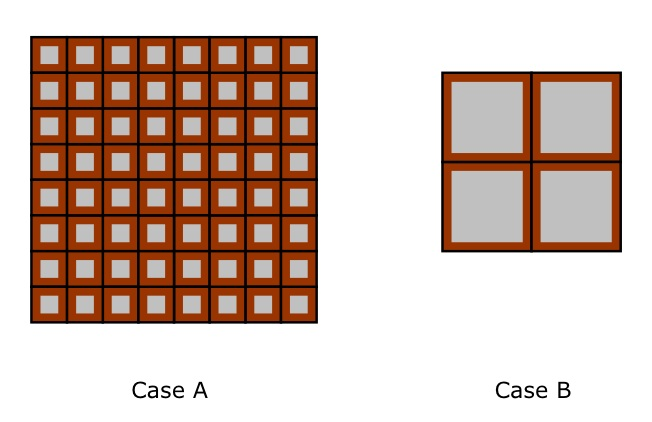
\includegraphics[scale=.65]{pic/Grainsize.jpg}
  \caption{Two different grainsizes.}
  \end{figure}

  In this illustration, light gray is the useful work that can be done and dark gray is the overhead needed to do this work. In cases like these a small grainsize is detrimental to the efficiency of the program. Parallel programming in any language requires the program to be slightly more attuned to nuances of the language.


  \section{Mutexes}
  Mutexes in TBB control how many threads can access a certain chunk of code at the same time. TBB includes six different types of mutexes, all of which behave in slightly different ways and are better for different cases. There are four traits that help to differentiate these mutexes. \todo{Elaborate all of these descriptions.}

  \begin{description}
  \item[Scalable] mutexes can help when dealing with heavy contention by forcing the process to never do worse then serial execution. The overhead from a non-serial mutex can in fact slow down the overall execution of the program. However, if the contention on the mutex is light, scalable mutexes can actually perform worse.
  \item[Fair] mutexes forces threads to execute in the order they arrived at the mutex. An unfair mutex is allowed to let running threads take precedence, which can speed up code.
  \item[Recursive] mutexes allow the thread that already owns the mutex to reacquire the same mutex again. This can be helpful for recursive functions, but can also make the locks much more complex.
  \item[Yield or Block] there are two options when it comes to what the mutex does while waiting. If the mutex yields, it repeated polls whether progress can be made. If it cannot, the mutex temporarily yields. If it blocks, it will yield until the mutex allows for progress.
  \end{description}

  \section{Atomics}
  Like CUDA, Intel TBB also has atomic functions. Also like CUDA, these functions only allow one thread to complete the given operation at a certain time. However, unlike CUDA in TBB atomics are not functions, but rather a data template. The \comp{atomic} template can be used with an integral, enumeration or pointer type. There are five functions provided:
  \begin{enumerate}
  \item Read
  \item Write
  \item Fetch and Store
  \item Fetch and Add
  \item Compare and Swap
  \end{enumerate}
  Exact syntax for these constructs can be found in TBB documentation. Use of these functions should be as closely monitored as any atomics, and they should be avoided if possible. 
  
  \section{Taks Scheduler}
  Another way that TBB gives the programmer more control over the final execution of the program is through the use of the \emph{task scheduler}. The task scheduler allows a programmer to explicitly define when a thread spawns child processes and how the parent thread combines the answers from those children. Although it is typically better to use the templates provided by TBB, the thread scheduler can be used to perform operations that are not provided.

  We'll take a look at some code provided by the TBB tutorial to see this in action.

  \lstinputlisting{code/TBBTaskScheduler.cpp}

  To run code:

  \lstinputlisting{code/RunTaskScheduler.cpp}

  Note that the parallel method includes a test for the size of data. If the data set is too small, it is a better decision to run the calculation in serial. Note how tasks are created in different ways dependent on whether or not it is the root process or a child process.

  \section{Conclusion}
  Note that unlike CUDA, we did not cover large amounts of code. This is because I spent a considerably larger amount of time working with CUDA and therefore, had a much larger body of code to comment upon.

\part{OpenMP}
OpenMP is the last parallel language we are going to cover. Parallelism is added into the code through the use of \emph{pragmas}, or small pieces of code that delimitate sections of the program to be run in parallel. OpenMP solutions tend to be easier to add into a program without needing to redesign the entire project. Small sections of code can be parallelized, and a speed up gained from these portions.

OpenMP is also unique in allowing for coding in language other than C++. OpenMP includes the ability to code in Fortran. The effect of the language is the same, but the exact syntax differs slightly. We will cover the language in C++ in order to maintain continuity throughout this document, but readers who are more comfortable with the Fortran language should look into the documentation.\footnote{\comp{https://computing.llnl.gov/tutorials/openMP/}}
	\section{Pragma}
	The pragma is the coding construct used by OpenMP to add parallelism into code. All pragmas follow the same general format: \comp{\#pragma omp directive-name [clause,...] newline}. There are many different \comp{directive-name}s allowed by the OpenMP language, which we will look at. The optional \comp{clause} argument is typically data scoping for threads. This allows the program to create private variables for each thread, or globally accessible variables that each thread is given access to. Let's take a look at an empty code example that shows the basic outline strategy of pragma code:
	
	\lstinputlisting{code/GeneralOpenMP.cpp}
	
	Now all that is left is filling the code out with functionality.
	
	\section{Fork-Join}
	OpenMP's parallel implementation is based on a fork-join model. All programs begin with a master thread which spawns teams of theads to complete parallel sections, until they all return, causing the master thread to continue with serial execution.
	
	\section{Standard Parallel Execution}
	Before we get into the oddities of the language, and the more complex constructs, let's take a look at a very simple piece of code that can solve a trivial example. In this program, we will randomly fill two arrays and then compute the sums of matching items in parallel.
	\todo{Comment this code}
	\lstinputlisting{code/OpenMPSimple.cpp} 
	
	The \comp{parallel omp for} directive tells the program that the following \comp{for} loop can be broken into multiple parts that can be run in parallel. The \comp{chunk} variable specifies the minimum grainsize for splitting the loop up. The \comp{dynamic} variable instructs the program to dynamically schedule the process execution upon running. This is the most simple directive that OpenMP has, but can be very helpful for implementing embarrassingly parallel problems.
	
	\section{Section Parallelism}
	A unique feature of OpenMP is its ability to perform \emph{section parallelism}. Until now, we've worked exclusively on data parallelism, which followed the general SIMT architecture. Section parallelism allows for the use of MIMD (Multiple-Instruction-Multiple-Data) to solve problems. In general, this would consist in a single parallel section executing several code blocks on a range of data simultaneously. 
	
	\lstinputlisting{code/SectionOpenMP.cpp}	
	
	Although this code does not perform any calculation, and we initialized no data, the construct should be readily understandable. The most important thing to remember when implementing section parallelism is that the process execution order is never guaranteed. Thus, sections computed in parallel should never depend upon the computations of the other, or modify results written by the other.     


    \section{Synchronization Constructs}
    Like most parallel languages, OpenMP contains constructs for synchronizing threads. OpenMP allows for nested constructs, which means that synchronization points are put inside parallel loops which means synchronization is added much like a parallel construct, using the same \comp{\#pragma omp} prefix. OpenMP allows for different constructs suck as \comp{critical}, \comp{barrier}, \comp{taskwait} and \comp{atomic}. These are used in a very similar manner to the synchronization commands used in other languages.
    
    \begin{description}
    	\item[Master] mandates that the following code can only be executed by the master thread.
    	\item[Critical] marks code that can only be executed by one thread at a time.
    	\item[Carrier] makes a point that all threads must reach before \emph{any} thread is allowed past the point.
    	\item[Taskwait] waits for child processes to complete before continuing execution.
    	\item[Atomic] marks memory locations that \emph{must} be accessed by only one thread at a time.
    \end{description}
    
    Like the use of any synchronization construct in \emph{any} parallel language, incorrect use of these directives can adversely affect code execution time due to threads blocking each other.   

\part{Extra Tools}
  \section{C++}
  All of the languages we have covered are mainly extensions to C++. I spent about a week of this summer reading about basic C++ so I would be better equipped to write code. There is no need to go into detail about the specifics of the language and there are many good books that can help. If you are going to spend any time working with any of these languages a solid understanding of C++ is a must. A lot of my previous knowledge was with Java which has a lot of similarities. The most difficult part for me was grasping how memory pointers and referencing works.

  \section{Git}
  We wont spend much time, but git is a very powerful tool for any programmer and I found it very helpful, so I'm going to explain how I as a single user utilize it and some of the commands that are helpful. Git is a decentralized version control tool that that is widely available for all major systems. There are many good guides that can explain the core concepts of git, which I would recommend. The tutorial I found most helpful was \comp{http://www.eecs.harvard.edu/\~{}cduan/technical/git/}

My work-flow tends to progress in a rather linear manner, but branches still come in very helpful. Whenever I begin a new problem I create a new repository with a branch that is the unaltered program so if everything goes wrong, I can always revert all my changes. The next important step is to divide the problem into the most logical steps and create a branch for each one. Typically if there are multiple files and each file has several main components I will begin a naming format such as: \comp{file.part} for each branch. I will also create a \comp{file.main} branch. After each smaller part is completed merge it into the \comp{main} branch. As each file is completed they are merged into a \comp{main} branch that has the most up to date and stable working release. Some important things to remember are commit often, it is cheap and you'll never know when you will want to go back to something that worked.

There are many other version control tools that are popular and work very well. I believe effective version control can make any programming experience better.

\section{Conclusion}


\nocite{*}

\bibliographystyle{plain}
\bibliography{sources}

\end{document}
